\documentclass[General-Information/Most_recent_log(3_0).tex]{subfiles}

\begin{document}
\subsection{There is only one Legendrian isotopy class.}
In all of these examples any newly added generators will be called $b_2$ and $b_1$ with $|b_1|+1=|b_2|$.
\subsubsection{Reidemeister 2}
\begin{example}
    \label{ex:1}
    Original trefoil is considered with a Reidemeister move 2 preformed in between crossings $a_5$ and $a_4$. Two generators $b_2$ and $b_1$ are created as undercrossings. 
    \begin{figure}[H]
        \centering
        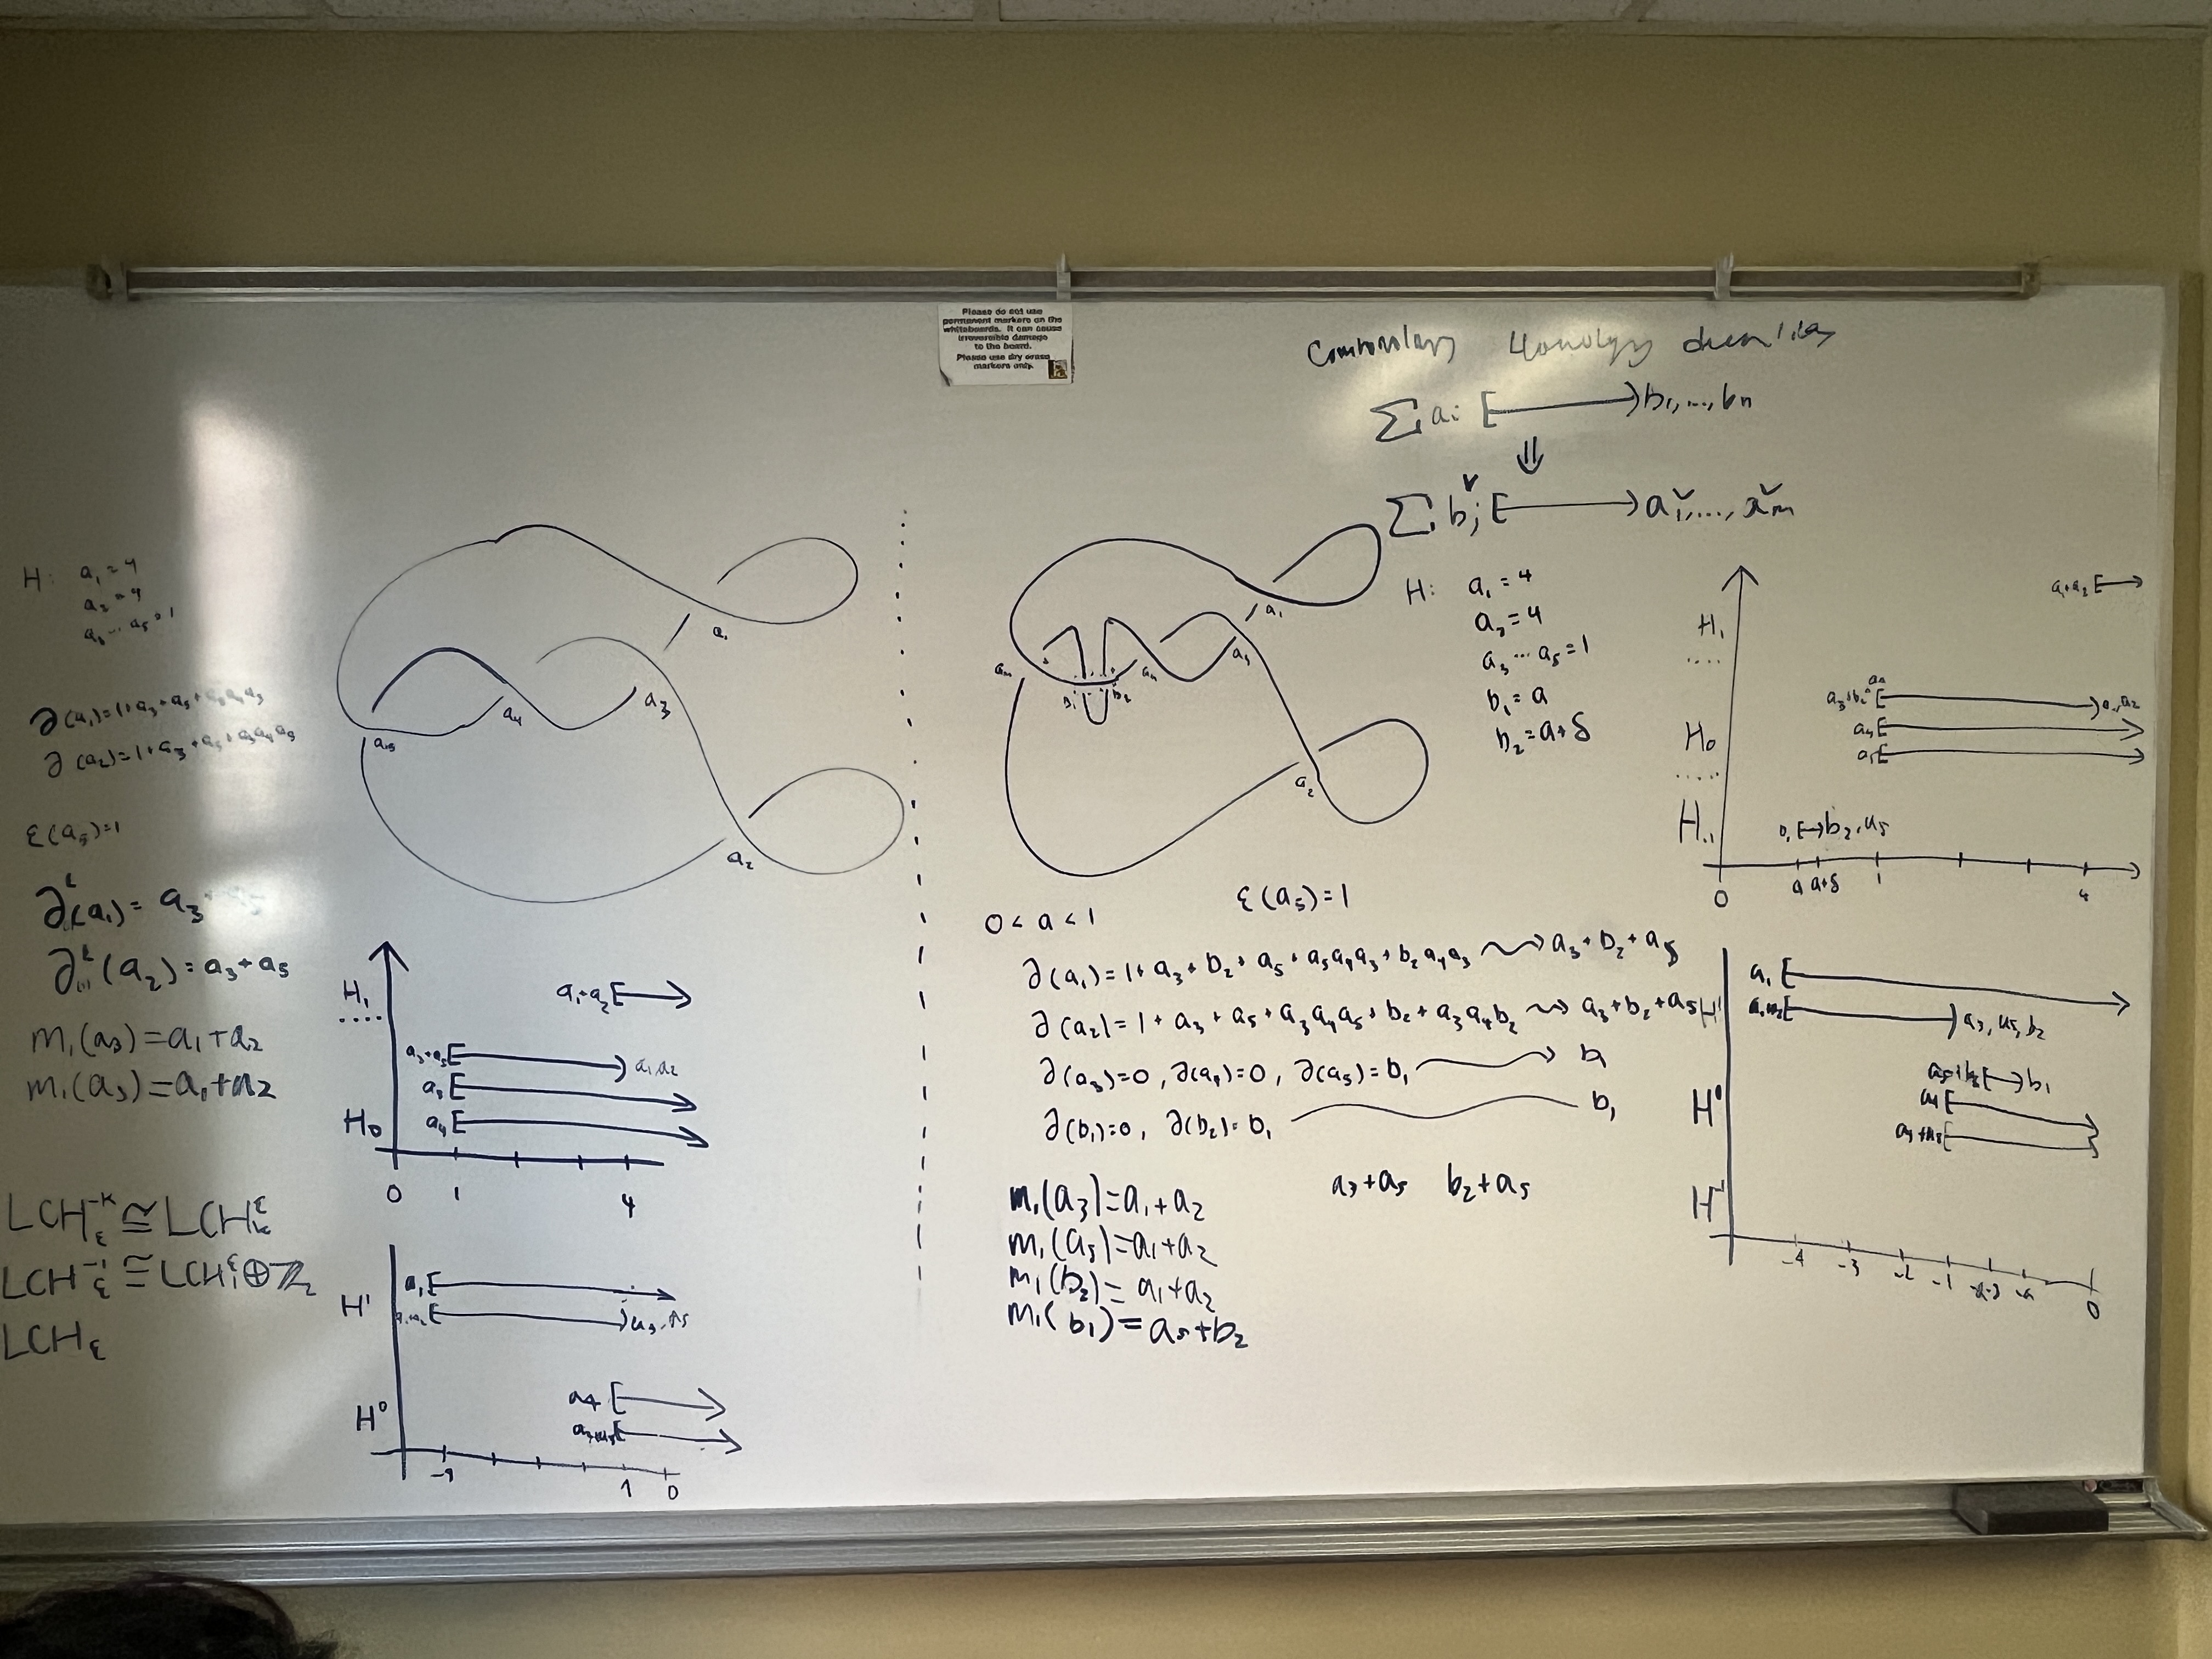
\includegraphics[width=\textwidth]{General-Information/Pictures/Examples/IMG-2747.JPG}
        \caption{Left: original trefoil and barcode. Right: trefoil after Riedemeister move 2 is preformed.}
    \end{figure}
\end{example}

\begin{example}
    \label{ex:2}
    Here a Reidemeister move 2 is preformed in between crossings $a_5$ and $a_4$, except now two overcrossings are added. Notice how in homology we have a finite bar $a_3+a_5$ now "pairing" with an infinite bar $a_3+a_5$ in cohomology. We wish to see how this pairing works in general for the rest of the examples. If we can show this pairing is preserved, then we know the finite bar in the trefoil is essential because the inifinite bar in cohomomology is essential, by functoriality.
    \begin{figure}[H]
        \centering
        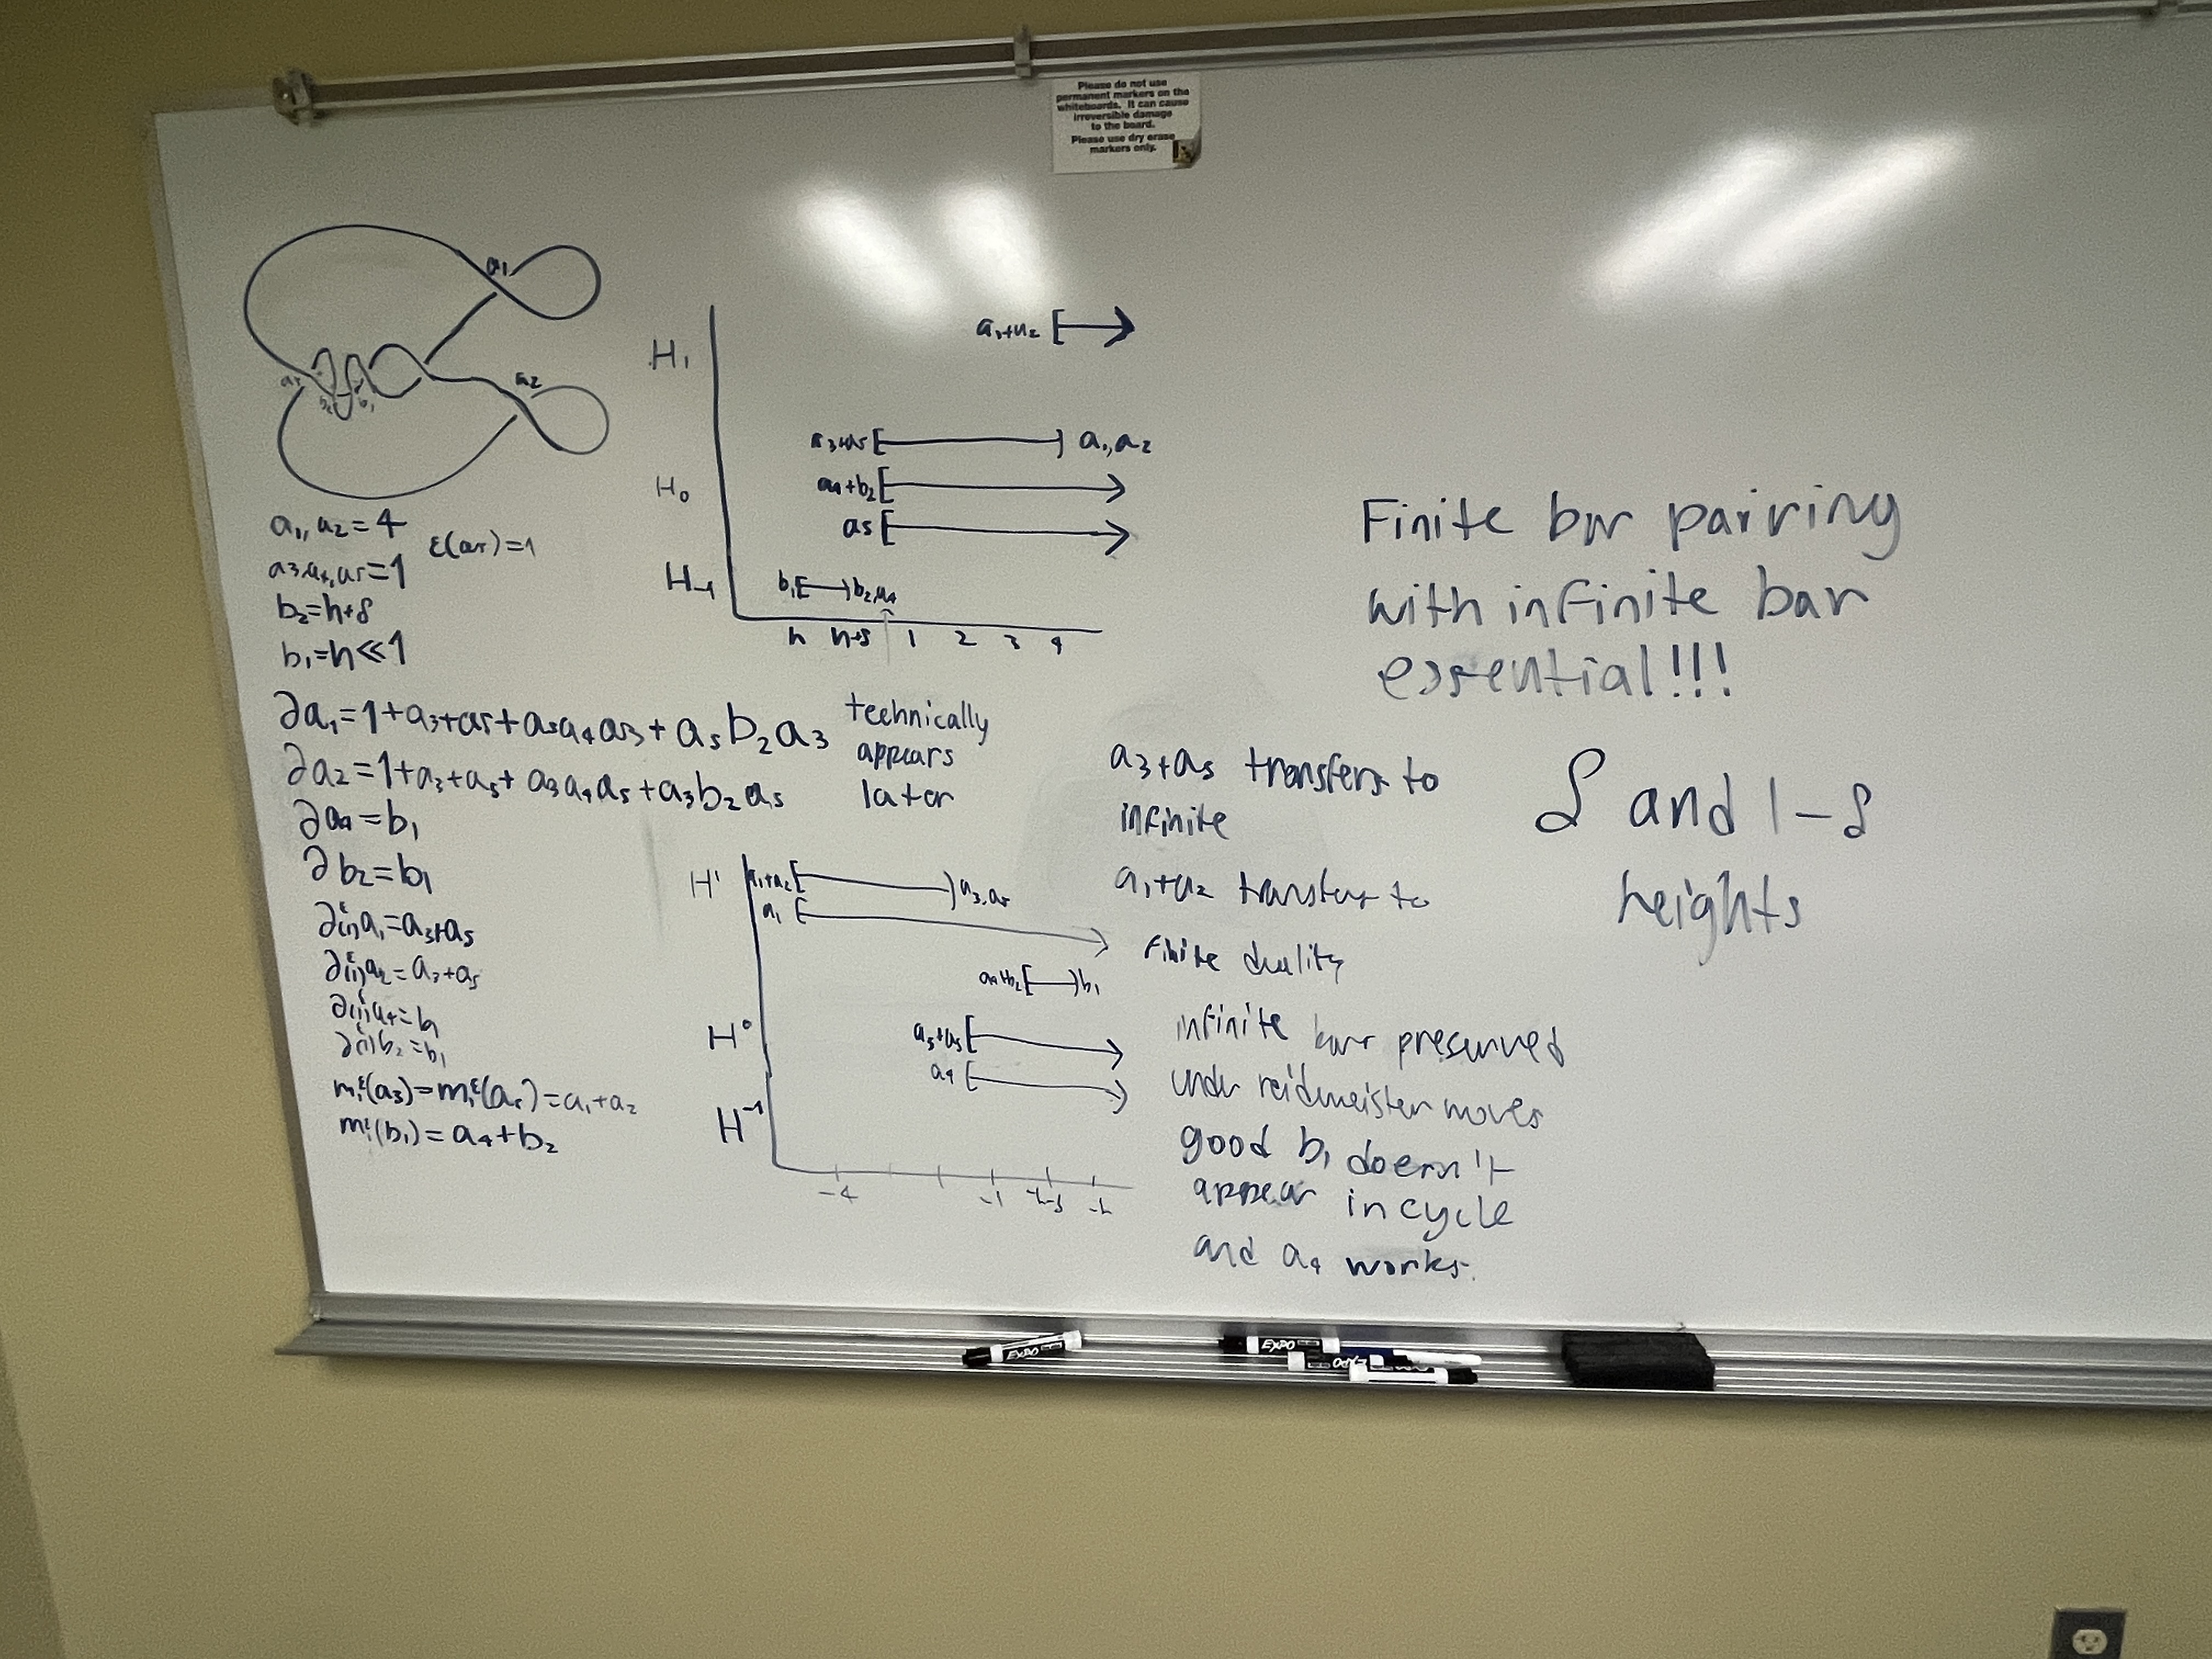
\includegraphics[width=\textwidth]{General-Information/Pictures/Examples/IMG-2751.JPG}
        \caption{Left: original trefoil and barcode. Right: trefoil after Riedemeister move 2 is preformed.}
    \end{figure}
\end{example}

\begin{example}
    \label{ex:3}
    Original trefoil is considered with a Reidemeister move 2 preformed in between crossings $a_5$ and $a_4$. See 
    \begin{figure}[H]
        \centering
        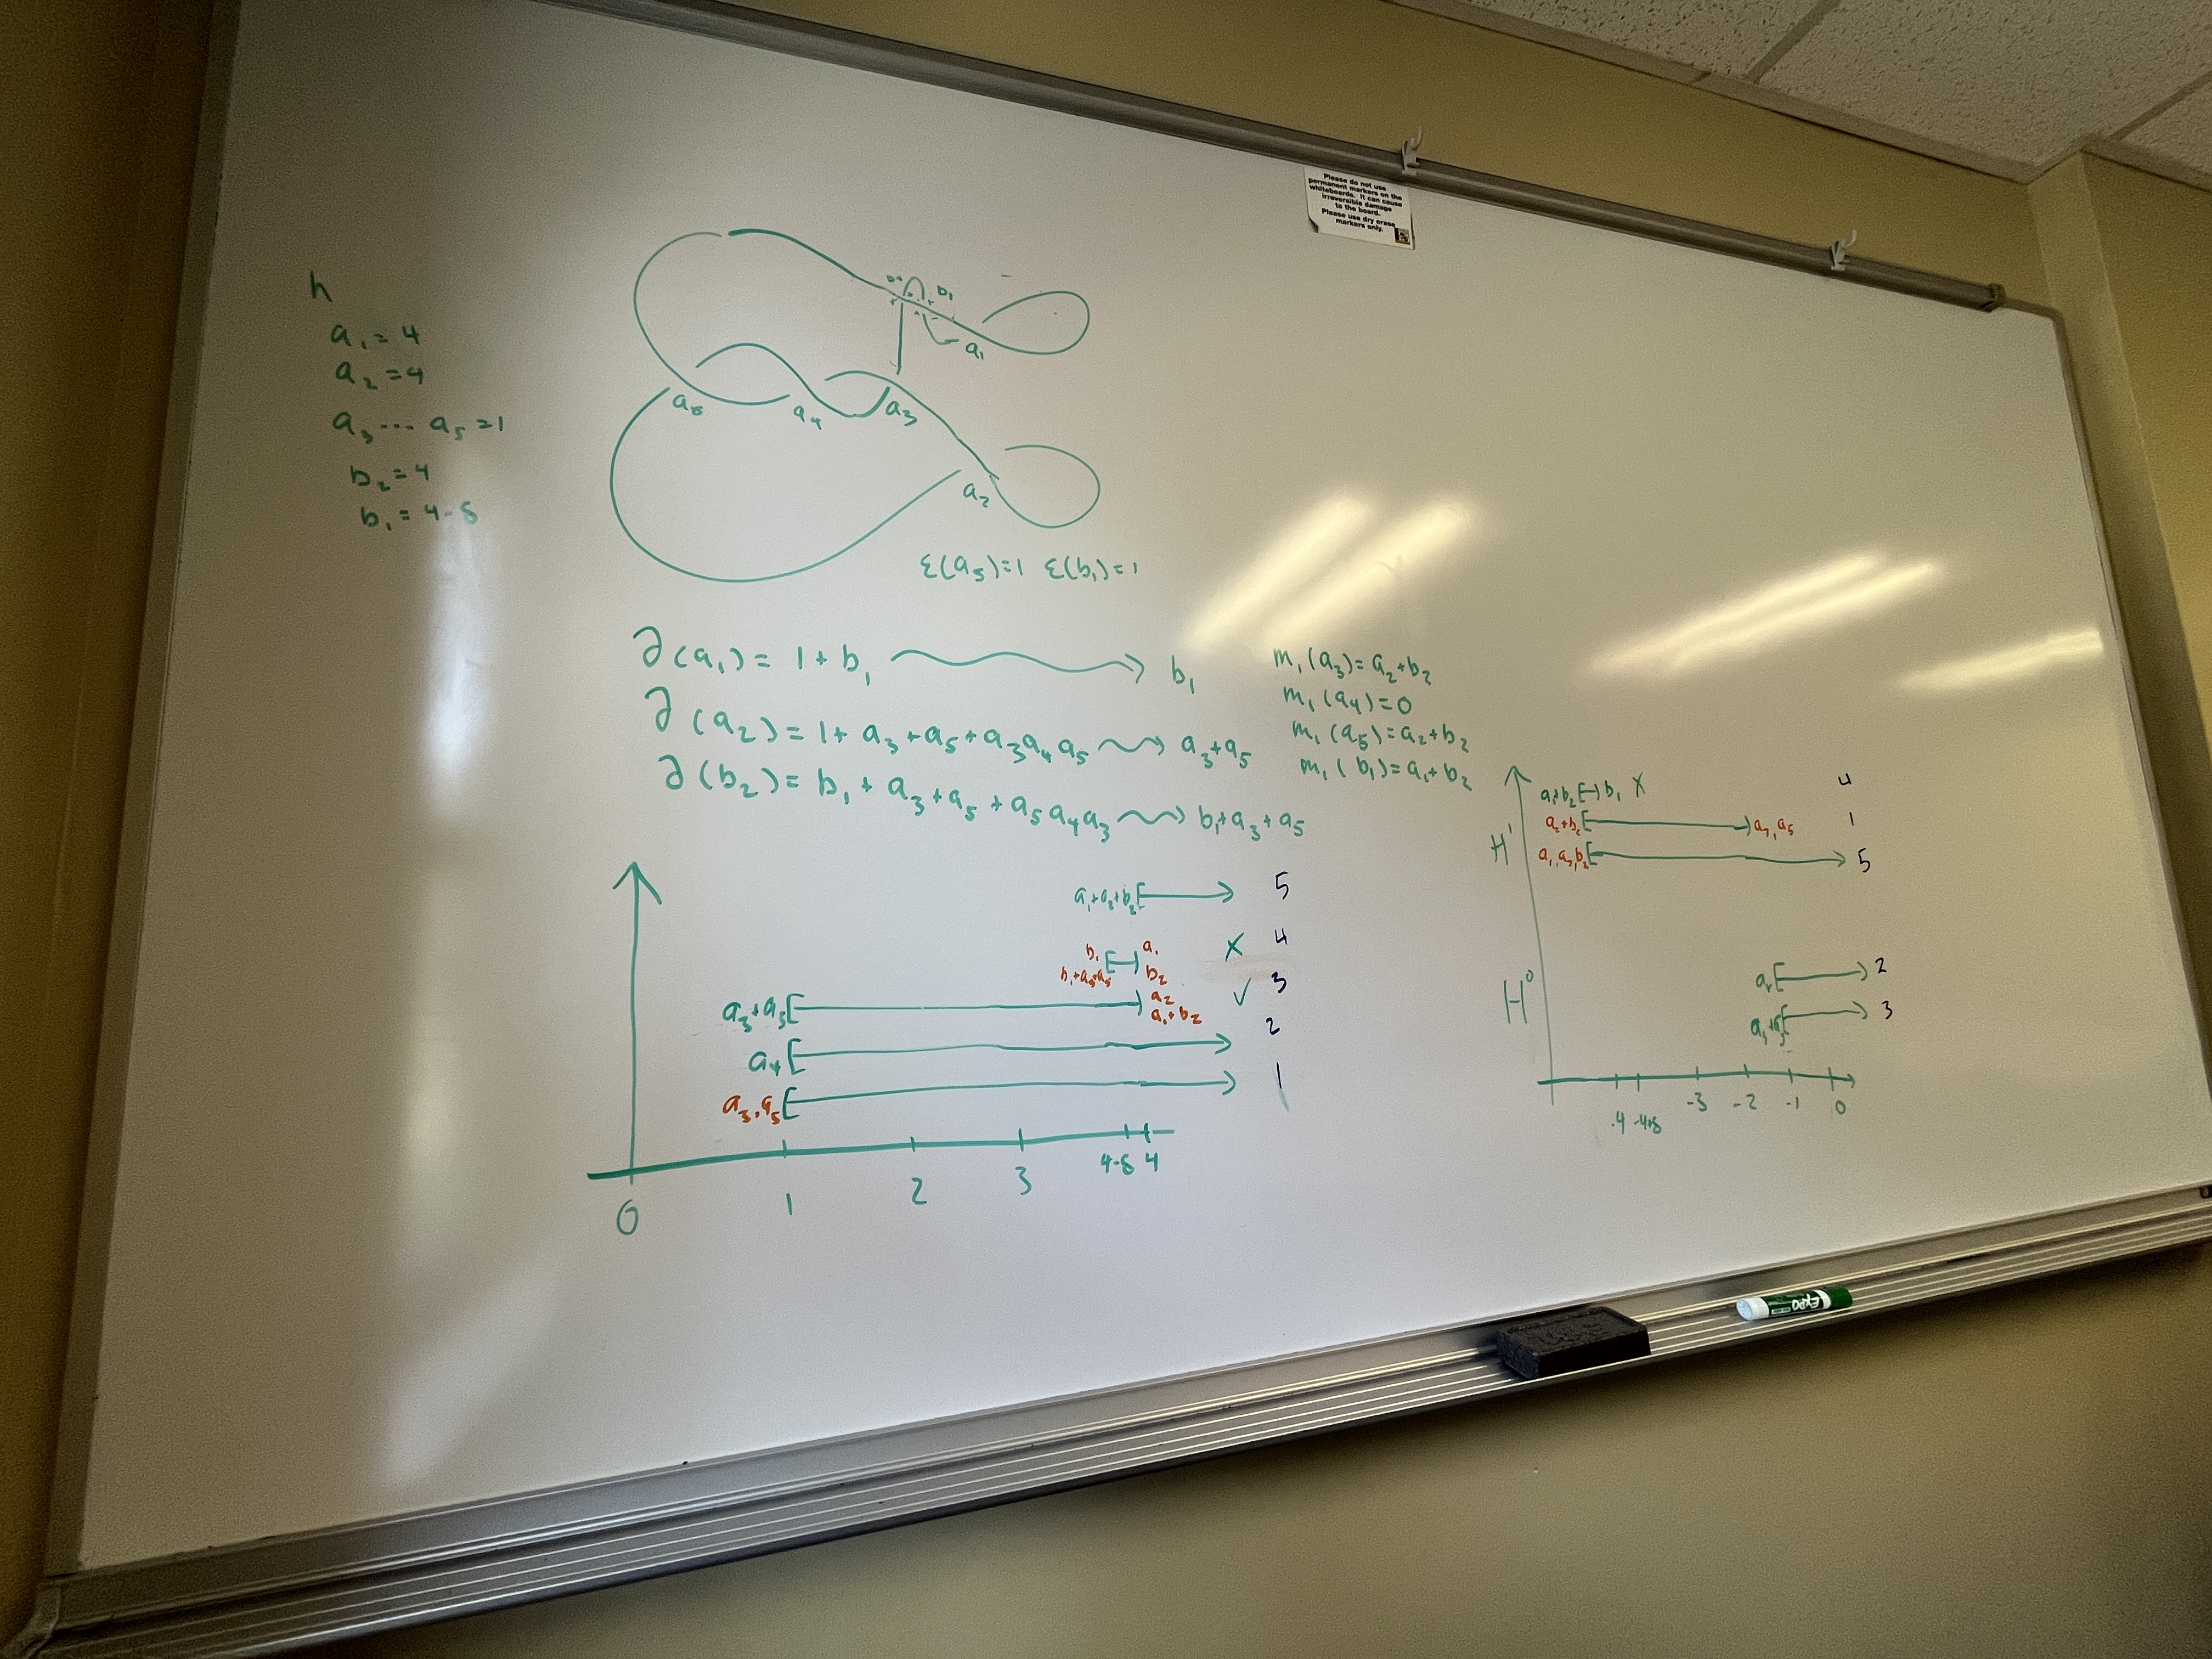
\includegraphics[width=\textwidth]{General-Information/Pictures/Examples/IMG-2754.JPG}
        \caption{Left: original trefoil and barcode. Right: trefoil after Riedemeister move 2 is preformed.}
    \end{figure}
\end{example}

\begin{example}
    \label{ex:4}
    Original trefoil is considered with a Reidemeister move 2 preformed in between crossings $a_5$ and $a_4$. See 
    \begin{figure}[H]
        \centering
        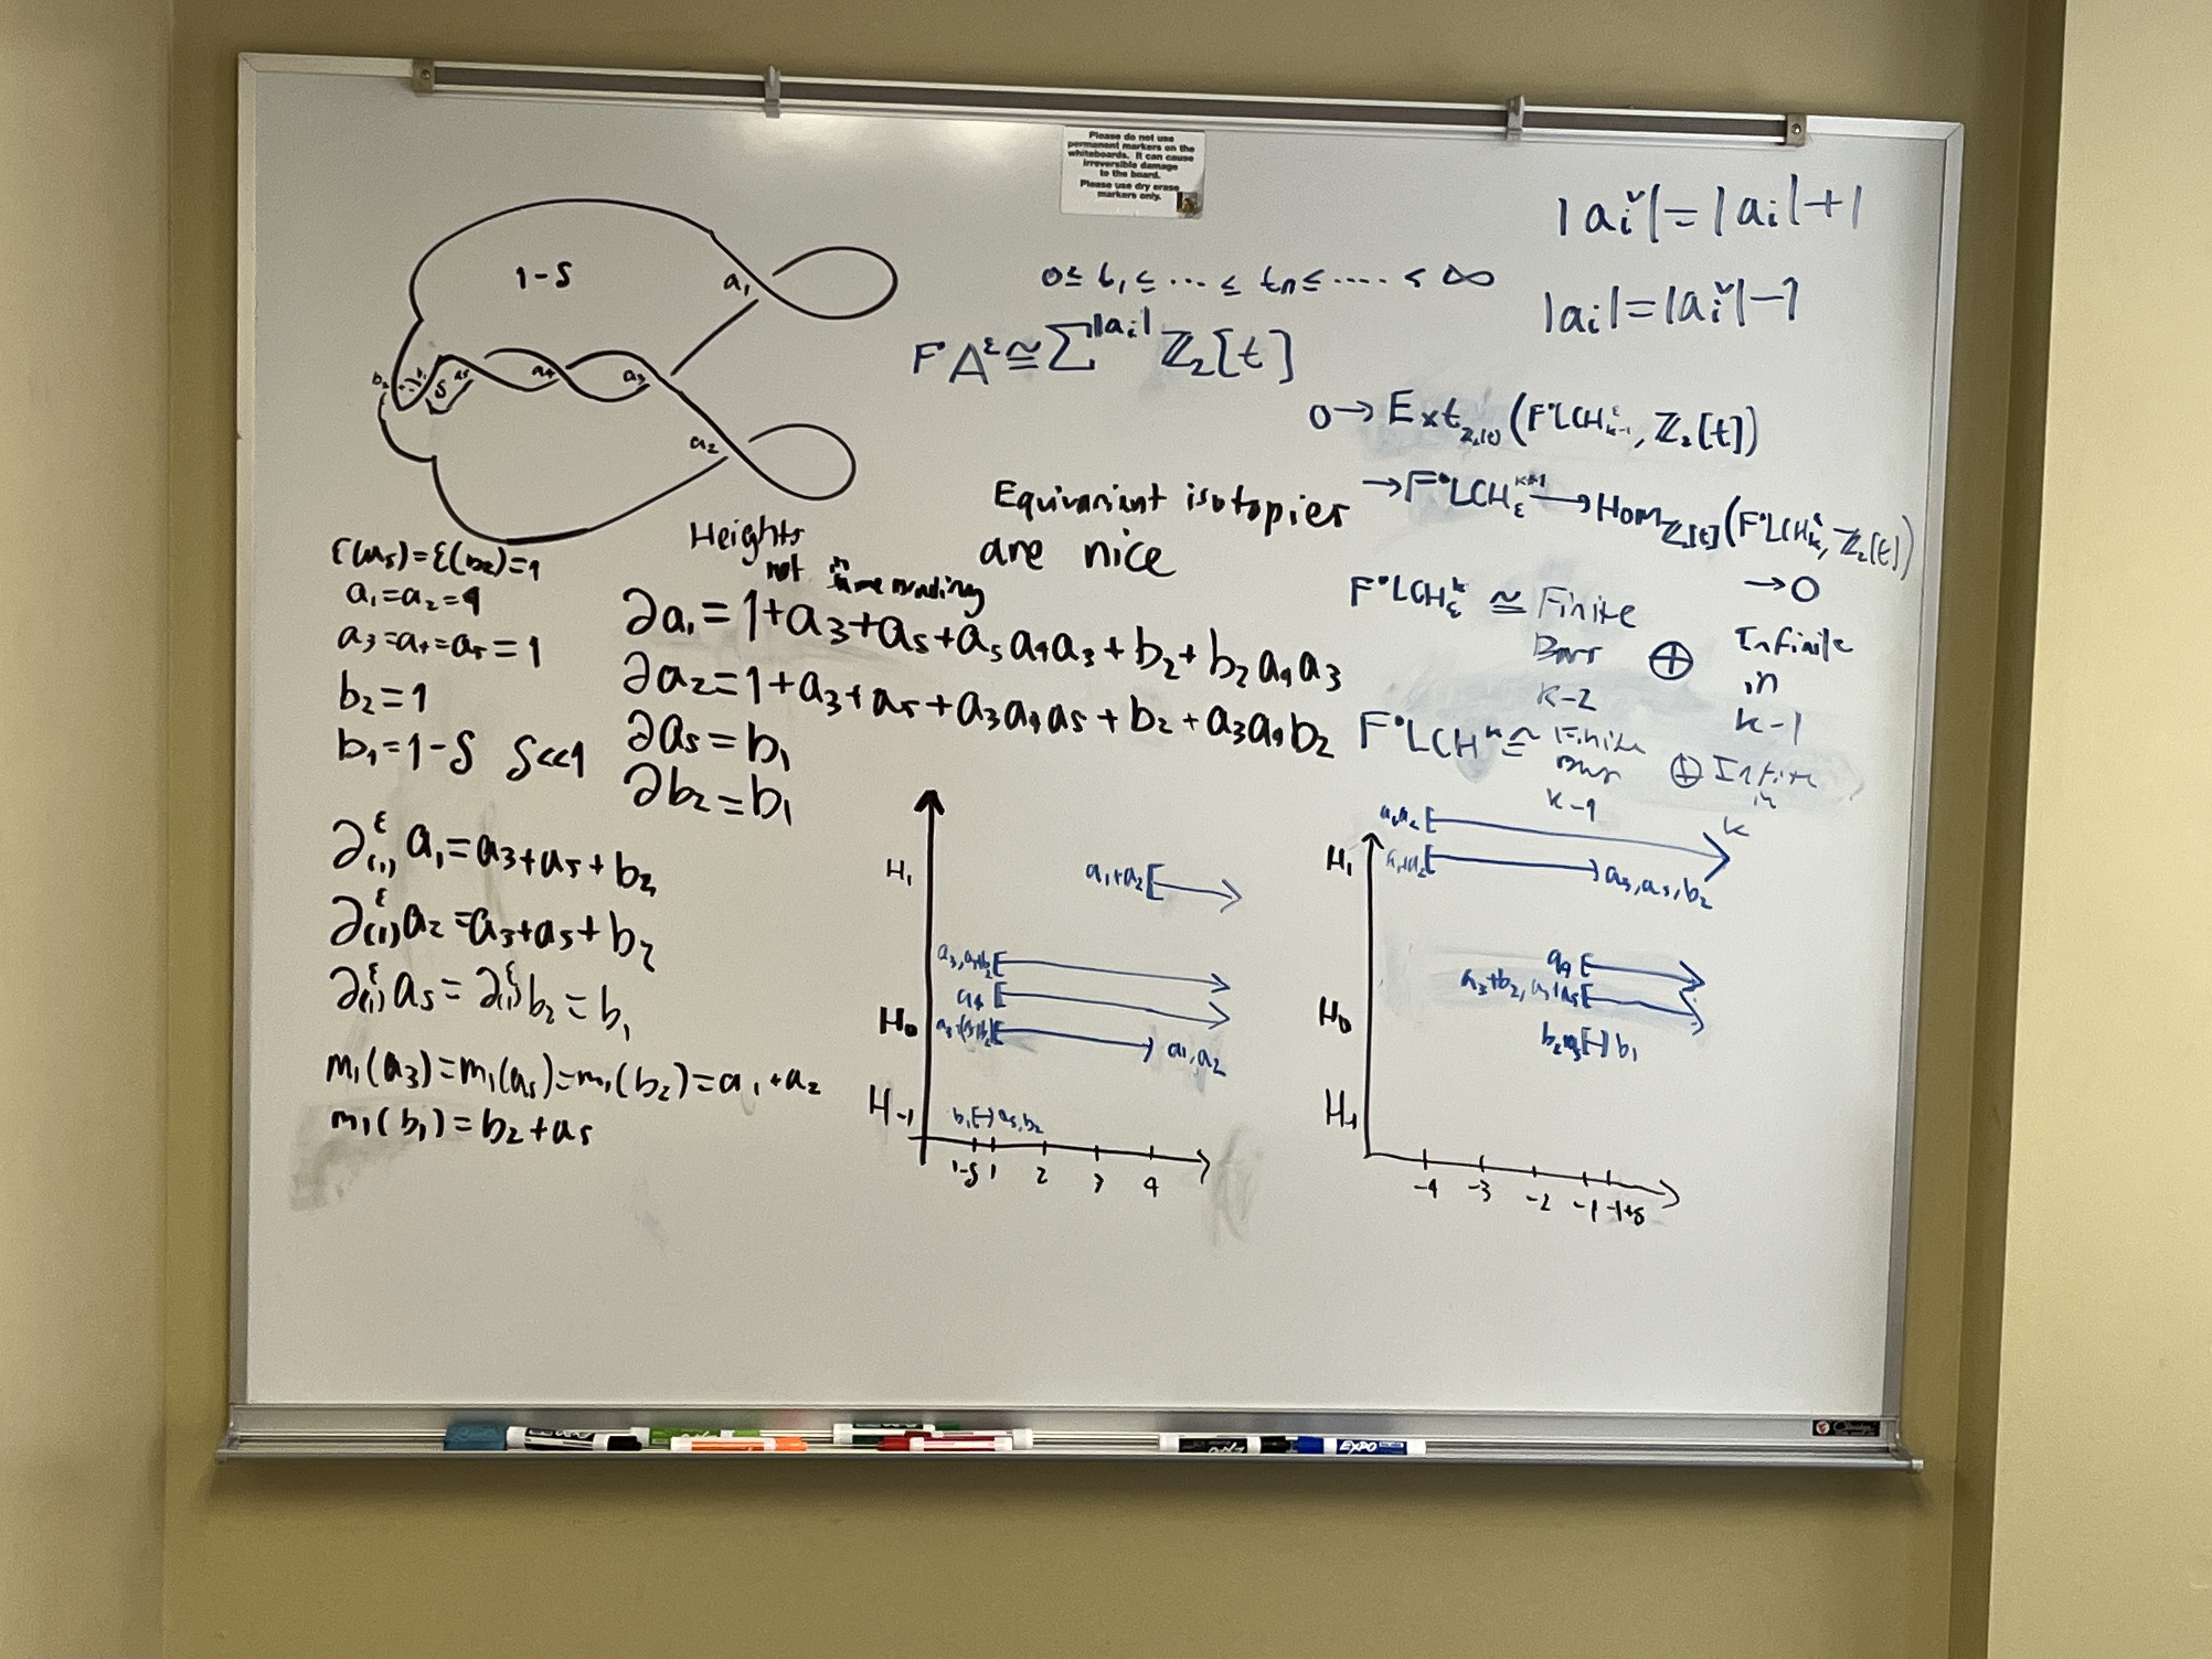
\includegraphics[width=\textwidth]{General-Information/Pictures/Examples/IMG-2758.JPG}
        \caption{Left: original trefoil and barcode. Right: trefoil after Riedemeister move 2 is preformed.}
    \end{figure}
\end{example}

\begin{example}
    \label{ex:5}
    Original trefoil is considered with a Reidemeister move 2 preformed in between crossings $a_5$ and $a_4$. See 
    \begin{figure}[H]
        \centering
        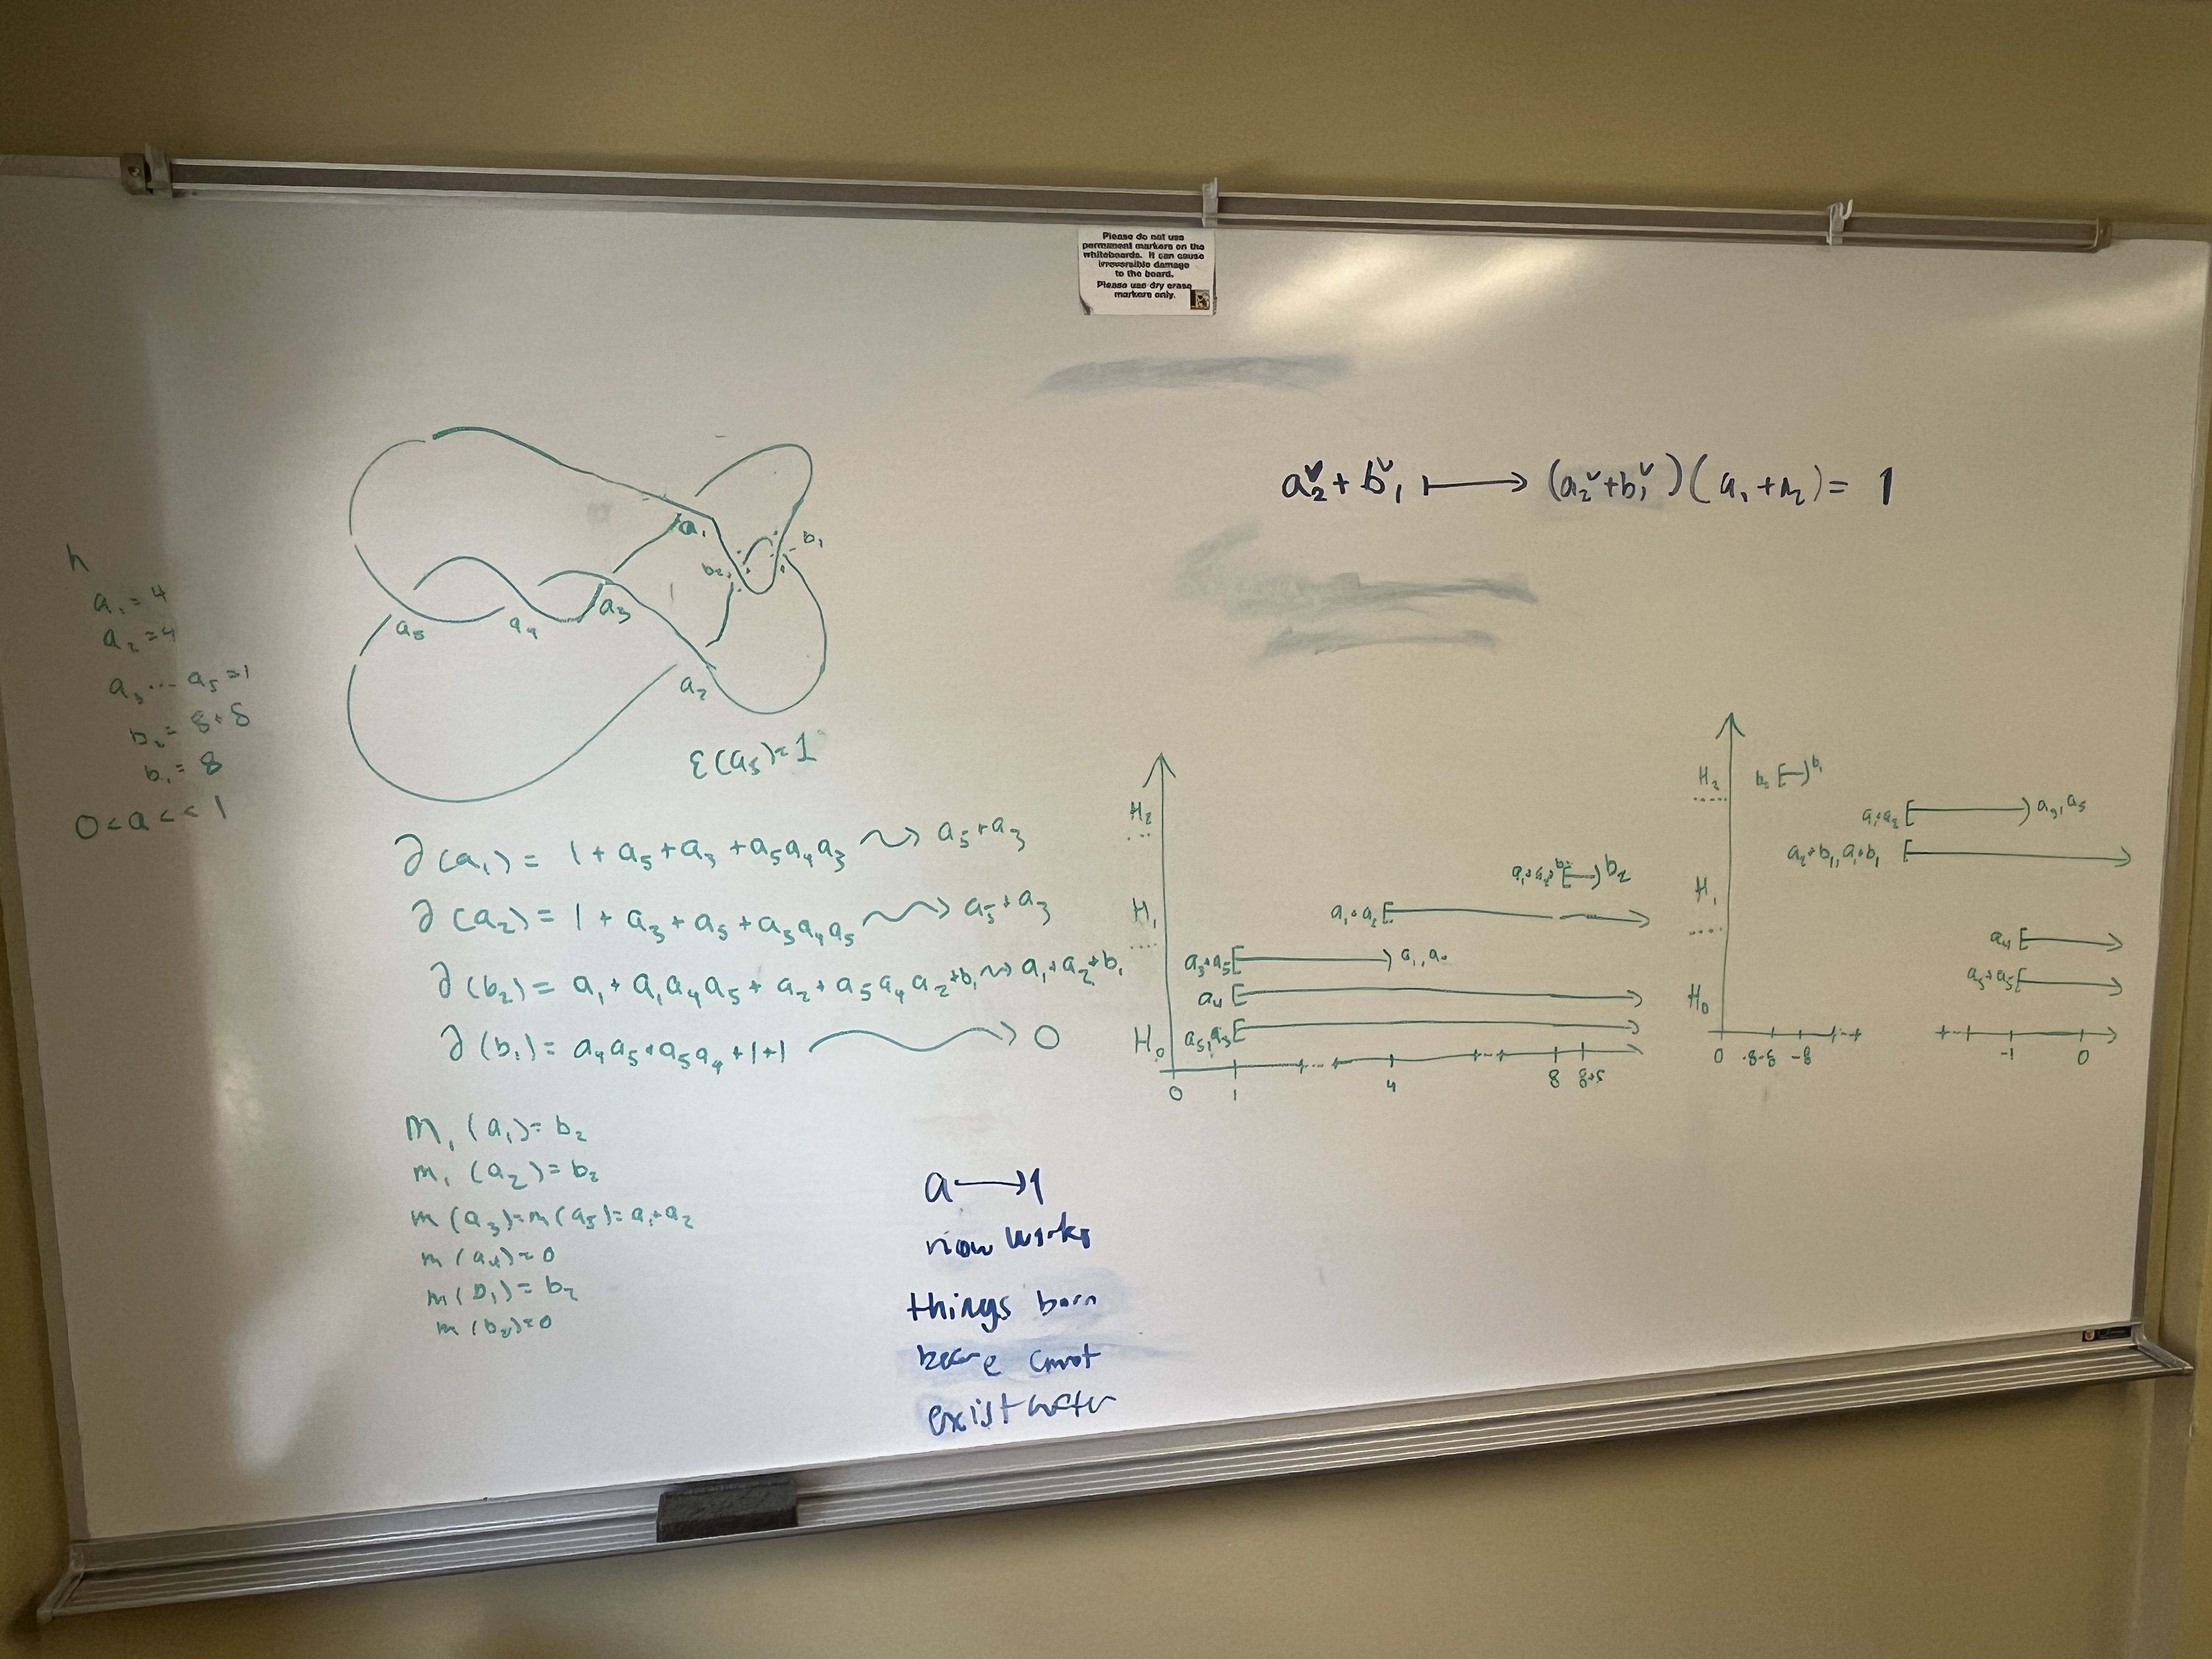
\includegraphics[width=\textwidth]{General-Information/Pictures/Examples/IMG-2759.JPG}
        \caption{Left: original trefoil and barcode. Right: trefoil after Riedemeister move 2 is preformed.}
    \end{figure}
\end{example}

\begin{example}
    \label{ex:6}
    Original trefoil is considered with a Reidemeister move 2 preformed in between crossings $a_5$ and $a_4$. See 
    \begin{figure}[H]
        \centering
        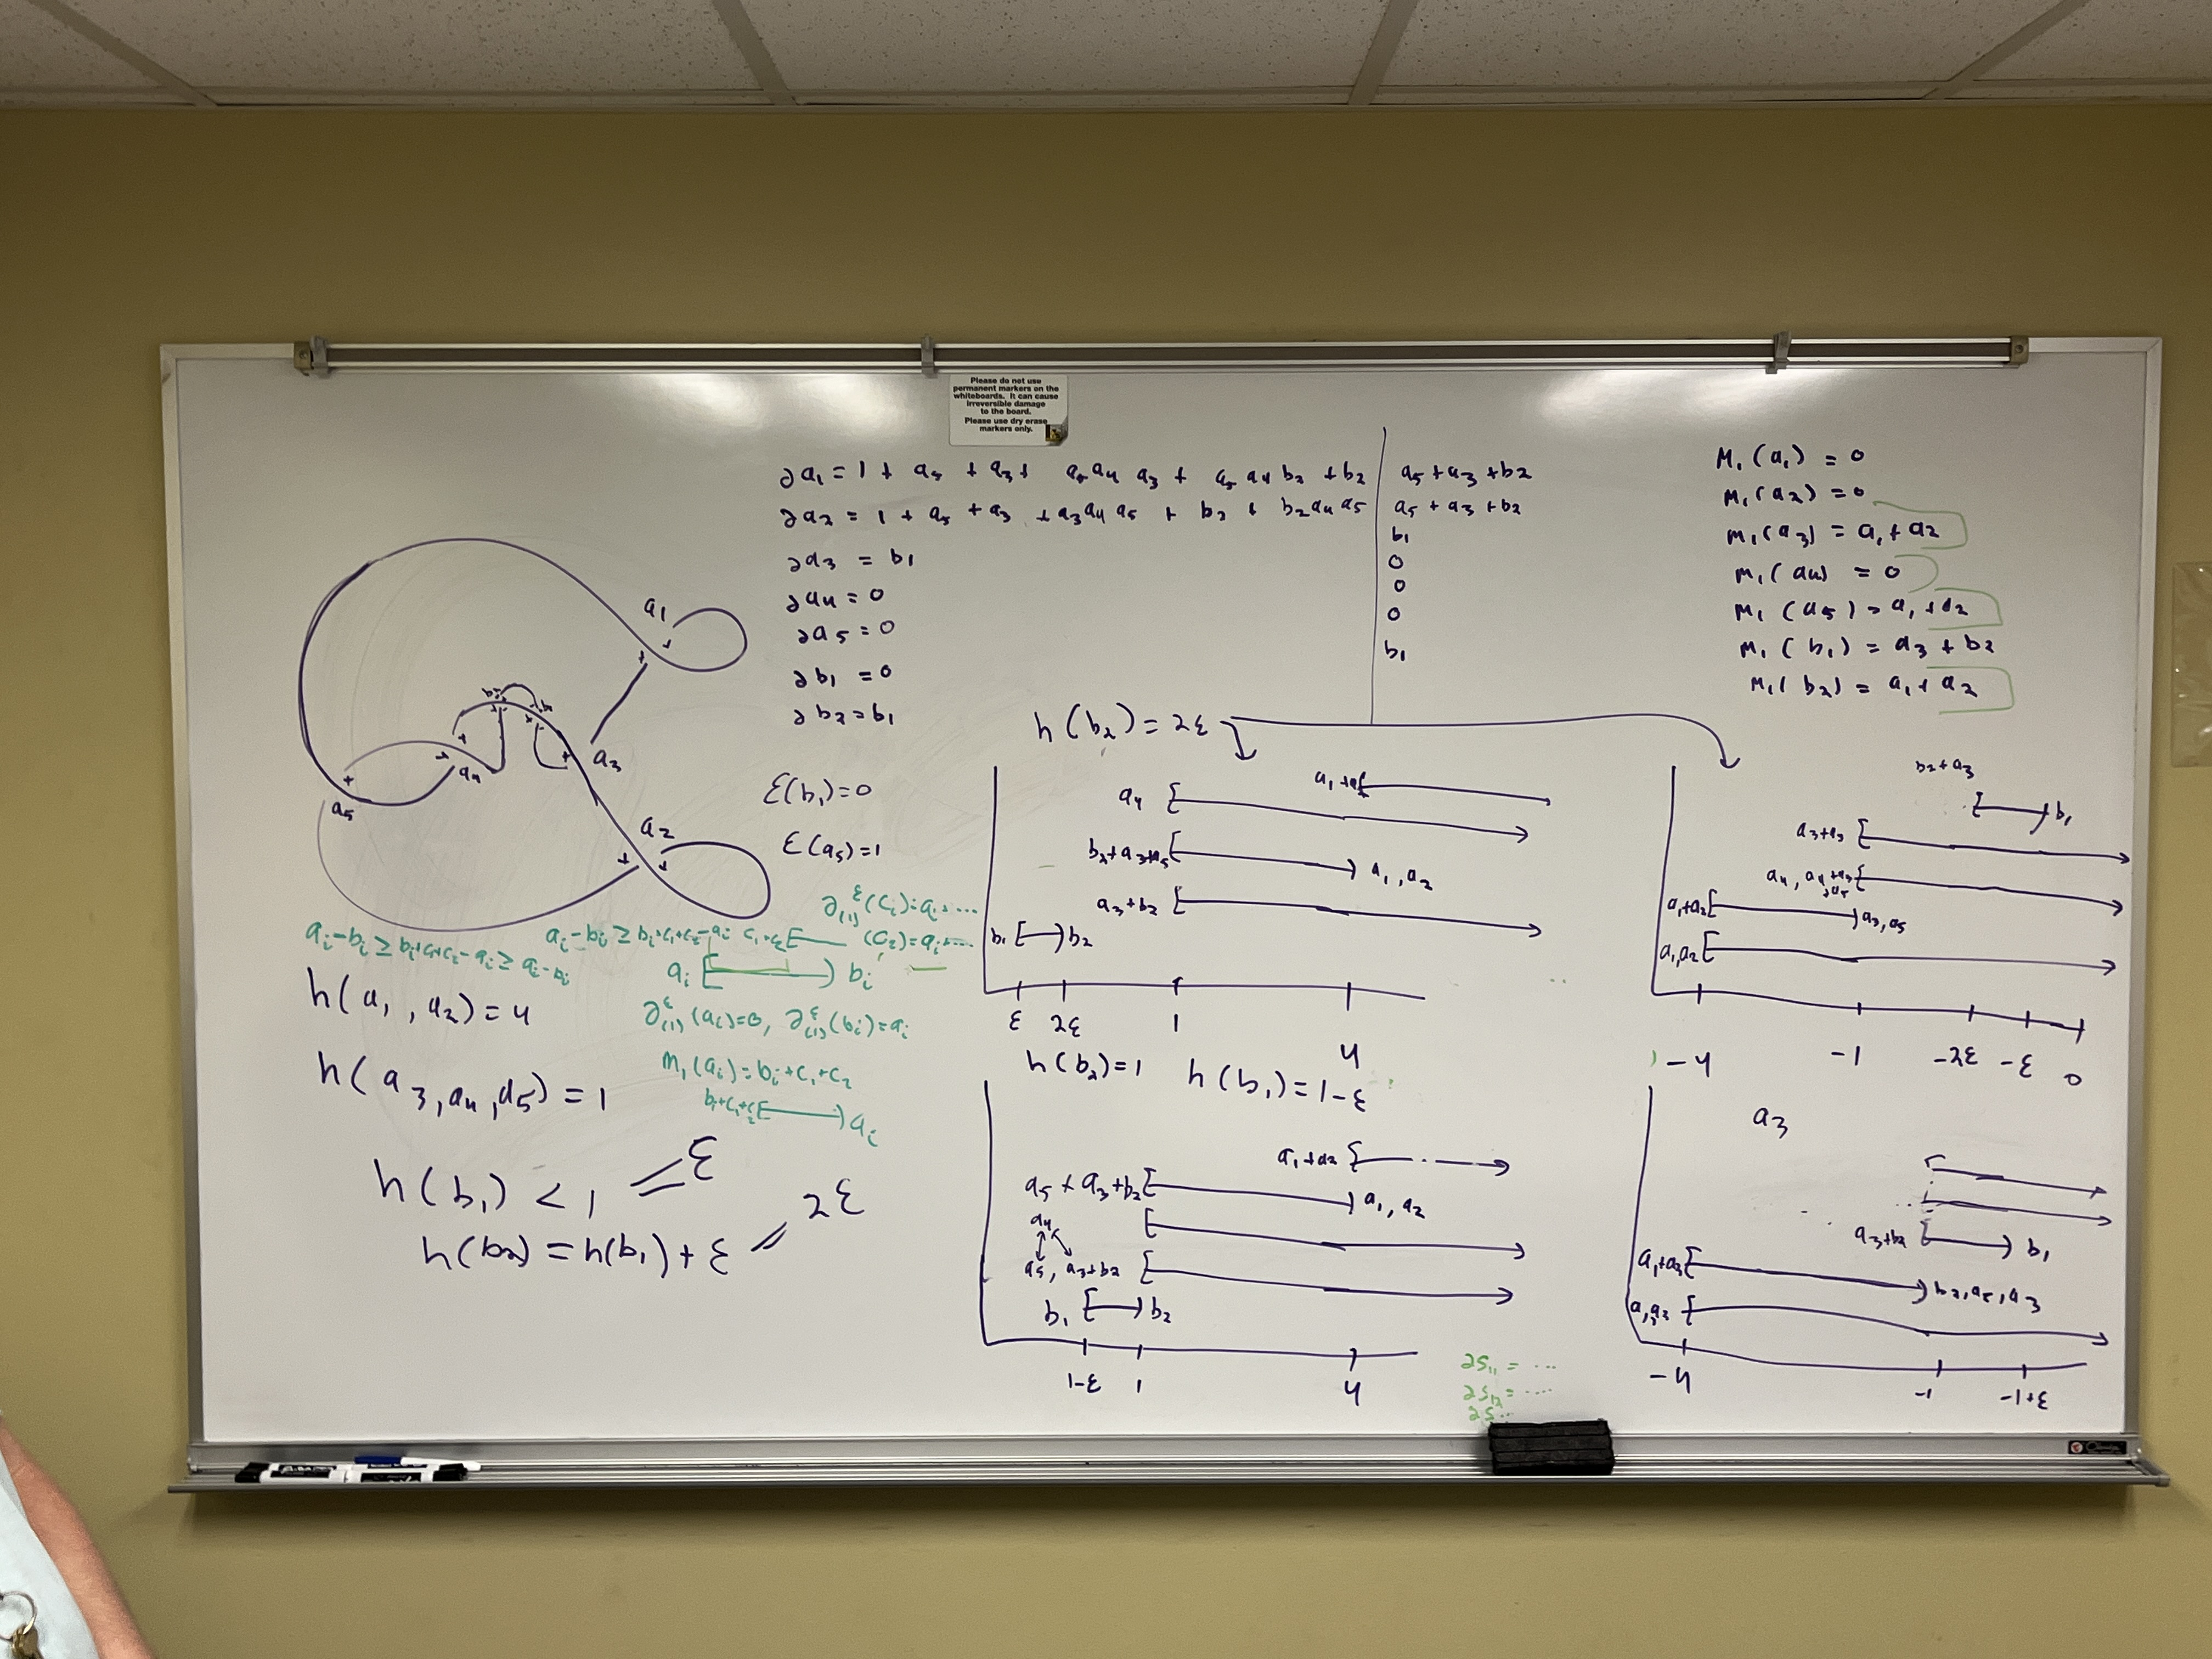
\includegraphics[width=\textwidth]{General-Information/Pictures/Examples/IMG-2760.JPG}
        \caption{Left: original trefoil and barcode. Right: trefoil after Riedemeister move 2 is preformed.}
    \end{figure}
\end{example}
\end{document}
